\section{Tiny Tapeout 2}
\label{sec:tinytapeout2}

\begin{figure}[!t]
\centering
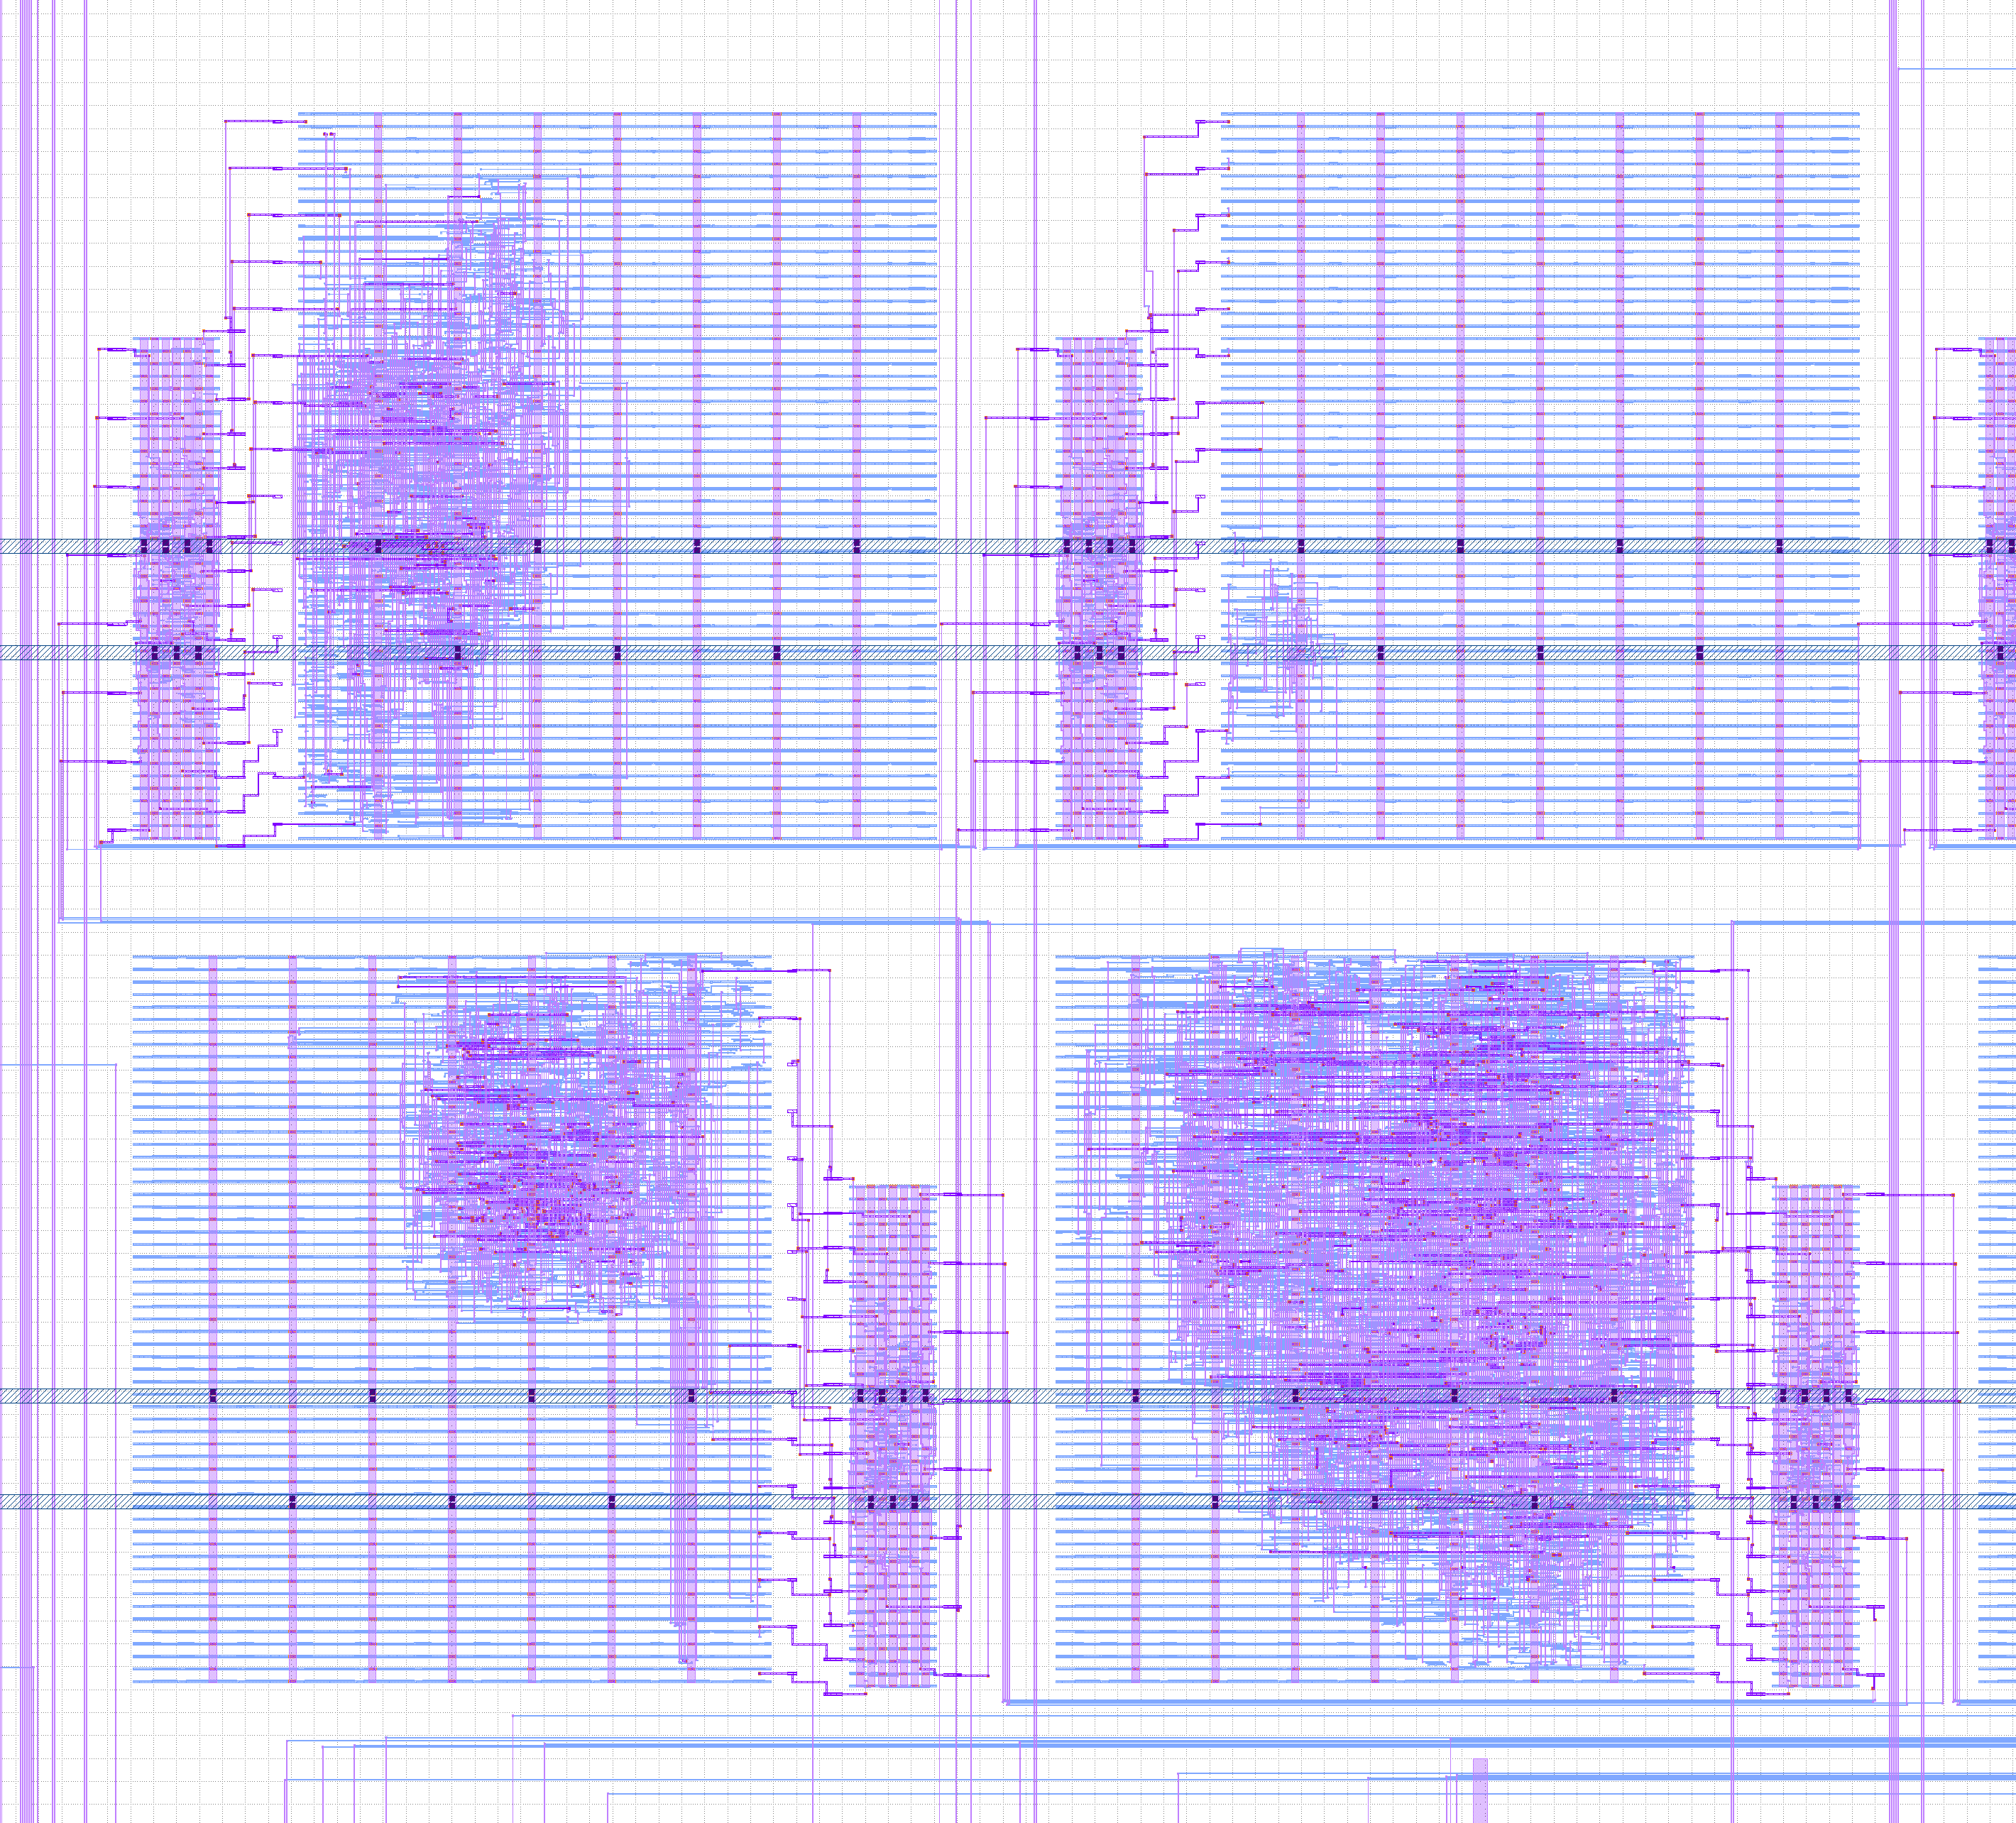
\includegraphics[width=\columnwidth]{./Figs/tt02_gds_zoom.png}
\caption{Tiny Tapeout 2 designs, showing the discrete scan chain blocks.}
\label{fig:TT02_separate_scan_blocks}
\end{figure}

After the concept had been proven, Tiny Tapeout 2 opened in November 2022 and 165 designs were submitted. This time, participants were charged and silicon manufacture was guaranteed. This was a big step forward, as until that time the only way to get guaranteed silicon with the open source PDKs was to pay for a full chipIgnite slot, costing \qty{10,000}{\$}. The finished design was submitted for fabrication on Efabless chipIgnite 2211Q.
To address the issue of accidental macro block removal encountered in Tiny Tapeout 1, Tiny Tapeout 2 moved the scan chain into a discrete macro block~\ref{fig:TT02_separate_scan_blocks}. This was present in all designs, and could not be modified by participants.

As with Tiny Tapeout 1, designs in in Tiny Tapeout 2 used two clock buffers, with the internal flops driven after the first buffer.

Tiny Tapeout 2 silicon was received in October 2023, tested for the first time on a public livestream, mounted on PCBs and sent to customers in January 2024.

%This needs to be expanded upon: what other changes were there in TT2? If there were no other changes, were there more participants in TT2 than TT1? Was anything else changed?
